\documentclass[10pt, a4paper]{article}
\usepackage{triada}

\graphicspath{{eps/}{png/}}

\renewcommand{\ell}{\mathcal{E}}

\usepackage{delim}
\usepackage{subfigure}
\usepackage{float}
                           
\begin{document}
\thispagestyle{empty}

\begin{center}
\ \vspace{-3cm}


\includegraphics[width=0.5\textwidth]{msu.eps}\\
{\scshape Московский государственный университет имени М.~В.~Ломоносова}\\
Факультет вычислительной математики и кибернетики\\
Кафедра системного анализа

%\vspace{5cm}
\vfill
{\LARGE Отчет по практикуму}

\vspace{1cm}

{\Huge\bfseries <<Динамическое программирование \\ и процессы управления>>}
\end{center}

\vspace{2cm}

\begin{flushright}
  \large
  \textit{Студент 415 группы}\\
  Д.~И.~Степенский

  \vspace{5mm}

  \textit{Руководитель практикума}\\
  асс. Ю.~Ю.~Минаева
\end{flushright}

\vfill

\begin{center}
Москва, 2012
\end{center}

\newpage

\tableofcontents

\newpage

\section{Постановка задачи}
Рассматривается следующая дискретная система:
\begin{equation}\label{statement_system} \begin{cases}
{x}(k+1) = A(k)x(k)+B(k)u(k),\quad k_0\leqslant k\leqslant k_1],\\
x(k_0)\in \ell(x_0,X_0), \\
u(k) \in \ell(q(k),Q(k)),\\
u(k)\in \mathbb{R}^m, x(k)\in \mathbb{R}^n.
\end{cases} \end{equation}  

Требуется построить внутреннюю эллипсоидальную оценку множества достижимости данной системы.

\section{Теоретическая часть}
\subsection{Множество достижимости}
%Вначале будем считать, что матрицы $B(i)Q(i)B(i)'$ и $A(i)$ несингулярны, т.е. имеют полный ранг. Случай сингулярных матриц будет разобран позднее.
\begin{df}
\textit{Эллипсоидом} $\ell(q,Q), Q\in\mathbb{R}^{n\times n}$ в $n$-мерном пространстве назовём множество точек
\[ \ell(q,Q) = \left\{ x\colon (x-q)'Q^{-1}(x-q) \leqslant 1 \right\}. \]
Здесь $q$ --- \textit{центр} эллипсоида, а $Q$ --- симметричная неотрицательно определенная \textit{матрица} эллипсоида. 
\end{df}
Эллипсоид назовем \textit{вырожденным}, если его матрица имеет неполный ранг, или, что равносильно, $\det Q = 0$.
\begin{df}
\textit{Множеством достижимости} дискретной системы, стартующей в момент $k_0$ из точки $x_0$ в момент времени $k$ называется следующее множество:
\[ \mathcal{X}(k,k_0,x_0) = \mathcal{X}[k] = \left\{ x \middle| \exists u(s), k_0\leqslant s\leqslant k\colon x(k|k_0,x_0)=x \right\}.\]
\end{df}
Понятие множества достижимости обобщается на случай произвольной стартовой точки из множества $\mathcal{X}_0$:
\[ \mathcal{X}(k,k_0,\mathcal{X}_0) = \left\{ x \middle| \exists u(s), k_0\leqslant s\leqslant k\colon x(k|k_0,x_0)\in \mathcal{X}_0 \right\} = \bigcup\limits_{x_0\in\mathcal{X}_0}\mathcal{X}(k,k_0,x_0).\]
\begin{theorem}
Решением системы \eqref{statement_system} является 
\begin{equation}\label{solution}
	x(k) = \Phi(k,k_0)x_0 + \sum\limits_{i=k_0}^{k-1}\Phi(k,i+1)B(i)u(i),
\end{equation} 
где $\Phi(k,p)$ --- переходная матрица:
\begin{equation}\label{solution}
	\Phi(k+1,p) = A(k)\Phi(k,p),\ \Phi(p,p)=I.
\end{equation}
\end{theorem}
\begin{proof}
	Докажем по индукции. Для $k=k_0+1$ очевидно. Пусть для $k$ показано, тогда для $k+1$
	проверим подстановкой в \eqref{statement_system}:
	\begin{gather*}
		{x}(k+1) = \Phi(k+1,k_0)x_0 + \sum\limits_{i=k_0}^{k+1-1}\Phi(k+1,i+1)B(i)u(i) = 
		\\ = A(k)\Phi(k,k_0)x_0 + A(k)\sum\limits_{i=k_0}^{k+1-2}\Phi(k,i+1)B(i)u(i) + 
		\Phi(k+1,k+1)B(k)u(k) = \\ = A(k)x(k) + B(k)u(k).
	\end{gather*}
\end{proof}
\begin{imp}
	Используя теорему, множество достижимости системы \eqref{statement_system} можно записать следующим образом:
	\begin{gather}
		\notag \mathcal{X}(k,k_0,\ell(x_0,X_0)) = q_c(k) + \Phi(k,k_0)\ell(0,X_0) + 
			\sum\limits_{i=k_0}^{k-1}\Phi(k,i+1)B(i)\ell(0,Q(i)) = \\
		= q(k) + \Phi(k,k_0)\ell(0,X_0) + 
			\sum\limits_{i=k_0}^{k-1}\Phi(k,i+1)\ell(0,B(i)Q(i)B(i)'),
	\end{gather}
	где \begin{gather}\label{ellipsoids_center}
		q_c(k) = \Phi(k,k_0)x_0 + \sum\limits_{i=k_0}^{k-1}\Phi(k,i+1)B(i)q(i).
	\end{gather}
\end{imp}
Здесь знак <<$+$>> означает сумму множеств по Минковскому: $A+B= \left\{x+y \middle| x\in A,\, y\in B\right\}$, а умножение множества на матрицу производится по формуле $\Phi A = \left\{ \Phi x\middle| x\in A \right\}.$ Кроме того, использовалось свойство эллипса $\Phi\ell(x,X) = \ell(\Phi x,\Phi X\Phi')$.
\subsection{Внутренние эллипсоидальные оценки}
Если умножение на невырожденную матрицу не выводит из класса эллипсоидов, то сумма двух эллипсоидов, вообще говоря, может не принадлежать этому классу, поэтому множество достижимости конкретным эллипсоидом записать не получится. Однако возможно эллипсоидальное оценивание этого множества.

Для начала найдем опорную функцию множества достижимости, пользуясь свойством её линейности относительно сумм по Минковскому, а так же тем, что опорная функция эллипсоида $\sufu{l}{\ell(x,X)}$ равна $\scalar{l}{x}+\norm{l}_X$:
\begin{gather}\label{th:ellipsoids_follow}
\notag\sufu{l}{\mathcal{X}\left(k,k_0,\ell\left(x_0,X_0\right)\right)} = \sufu{l}{q_c\left(k\right)} + \sufu{l}{\Phi\left(k,k_0\right)\ell\left(0,X_0\right)} +\\ 
			\notag + 
			 \sum\limits_{i=k_0}^{k-1}\sufu{l}{\Phi\left(k,i+1\right)B\left(i\right)\ell\left(0,Q\left(i\right)\right)} = 
			 \scalar{l}{q_c\left(k\right)} + 
				\sufu{l}{\ell\left(0,\Phi\left(k,k_0\right)X_0\Phi\left(k,k_0\right)'\right)} + \\
			\notag +\sum\limits_{i=k_0}^{k-1} 
				\sufu{l}{
					\ell\left(0,\Phi\left(k,i+1\right)B\left(i\right)Q\left(i\right)B\left(i\right)'\Phi\left(k,i+1\right)'\right)} = 
			 \scalar{l}{q_c\left(k\right)} +\\+ \scalar{l}{\Phi\left(k,k_0\right)X_0\Phi\left(k,k_0\right)'l}^{1/2}
			  +
			\scalar{l}{\Phi\left(k,i+1\right)B\left(i\right)Q\left(i\right)B\left(i\right)'\Phi\left(k,i+1\right)'l}^{1/2}.
\end{gather}
Заметим, что если предположить, что центры всех эллипсов нулевые, то из \eqref{th:ellipsoids_follow} исчезнет лишь первое слагаемое.
\begin{theorem}\label{th_st:internal}
Эллипсоид, являющийся внутренней оценкой суммы $\ell(0,Q_1)+\dots+\ell(0,Q_n)$, имеет матрицу
\begin{equation}\label{th:ell} Q = Q_*'Q_*,\quad Q_*=\sum\limits_{1}^{n} S_kQ_k^{1/2},\ S_kS'_k=I, \end{equation}
причем для оптимальности (в смысле касания заданного множества в направлении $l$) необходима и достаточна линейная зависимость векторов $S_kQ_k^{1/2}l,\ k=1,\dots,n.$
\end{theorem}
\begin{proof}
Для доказательства внутренности оценки достаточно показать, что опорная функция эллипсоида с матрицей \eqref{th:ell} всюду не больше опорной функции суммы эллипсоидов. Сравним квадраты опорных функций, пользуясь неравенством Коши-Буняковского:
\begin{gather*}
	\sufu{l}{\ell(0,Q)}^2 = \scalar {l}{\left( \sum\limits_{k=1}^{n}S_k Q_k^{1/2} \right)'\left( \sum\limits_{k=1}^{n}S_k Q_k^{1/2} \right)l} = 
	\sum\limits_{k=1}^{n}\scalar{l}{Q_kl} +  \\
		+ 2\sum\limits_{k=1}^{n} \sum\limits_{p=k+1}^{n}\scalar{S_kQ_k^{1/2}l}{S_pQ_p^{1/2}l} 
	\leqslant \sum\limits_{k=1}^{n}\scalar{l}{Q_kl} + 
		2\sum\limits_{k=1}^{n} \sum\limits_{p=k+1}^{n}\scalar{l}{Q_kl}^{1/2}\scalar{l}{Q_pl}^{1/2} = \\
	= \left( \sum\limits_{k=1}^{n}\scalar{l}{Q_kl}^{1/2} \right)^2 
	= \sufu{l}{\sum\limits_{k=1}^{n} \ell\left(0,X_k\right)}^2.
\end{gather*}
Равенство в неравенстве Коши-Буняковского, то есть оптимальность в смысле касания, достигается тогда и только тогда, когда линейно зависимы векторы $S_kQ_k^{1/2}l$.
\end{proof}

Из описанного выше следует теорема об аппроксимации множества достижимости системы \eqref{statement_system}.
\begin{theorem}
Для каждого момента времени $k$
\[\mathcal{X}\left(k,k_0,\ell\left(x_0,X_0\right)\right) = 
	\bigcup\limits_{l}\ell\left( q_c(k), Q(k,l) \right), \]
	где $Q$ задается \eqref{th:ell}, $q_c(k)$ задается \eqref{ellipsoids_center}, и 
	\begin{equation}
		Q_*(l) = \left( \left(SX_0S'\right)^{1/2} + \sum\limits_{k_*=k_0}^{k-1}S_{k_*}\left(\Phi(k_0,k_*+1)B(k_*)Q(k_*)B(k_*)'\Phi(k_0,k_*+1)'\right)^{1/2} \right) 
		\Phi(k,k_0)'
	\end{equation}
\end{theorem}
\begin{proof}
	Так как для касания по направлению $l$ требуется линейная зависимость $S\left(\Phi\left(k,k_0\right)X_0\Phi\left(k,k_0\right)'\right)^{1/2}l$ и $S_{k_*}\left(\Phi\left(k,k_*+1\right)B\left(k_*\right)Q\left(k_*\right)B\left(k_*\right)'\Phi\left(k,k_*+1\right)'\right)^{1/2}l$  (где $S$ и  $S_{k_*}$ ортогональны) для всех $k_0 \leqslant k_* \leqslant k-1$, то по ортогональной $S$ (например, $S=I$) можно получить из выражения все нужные линейно зависимые векторы, и при таком определении они будут удовлетворять условию равенства в неравенстве Коши-Буняковского из теоремы \ref{th_st:internal}. Поэтому, вообще говоря, внутренние приближения зависят лишь от $l$.

Доказательство самой теоремы теперь проведем двусторонним вложением. Имеем вложенность правой части условия в левую, поскольку все оценки --- внутренние. Вложенность же левой в правую получается из следующих соображений: для произвольного $x \in \mathcal{X}\left(k,k_0,\ell\left(x_0,X_0\right)\right)$ рассмотрим вектор $l = x - q_c(k)$. Для такого $l$ существует внутренняя эллипсоидальная оценка, которая касается $\mathcal{X}\left(k,k_0,\ell\left(x_0,X_0\right)\right)$ по направлению $l$. Но тогда эта оценка содержит весь отрезок от $q_c(k)$ до точки касания, а точка $x$ лежит на этом отрезке, а значит, принадлежит и правой части.
\end{proof}
\begin{note}
Заметим, что везде выше использовалось лишь свойство корня симметричной матрицы $Q^{1/2}\left(Q'\right)^{1/2} = Q$, поэтому мы вправе (то есть выкладки не изменятся) определить квадратный корень из матрицы $S$, как матрицу $S^{1/2}$ такую, что $S^{1/2}\left(S'\right)^{1/2} = S$.
\end{note}
Теперь можно записать более краткий вид корней описанных в теореме матриц: 
\begin{gather}
	\label{root_formula1} S\left(\Phi\left(k,k_0\right)X_0\Phi\left(k,k_0\right)'\right)^{1/2}l =
		SX_0^{1/2}\Phi(k,k_0)'l, \\ 
		\notag  S_{k_*}\left(\Phi\left(k,k_*+1\right)B\left(k_*\right)Q\left(k_*\right)B\left(k_*\right)'\Phi\left(k,k_*+1\right)'\right)^{1/2}l 
		= {}\\   \label{root_formula2} {} = S_{k_*}\left(B(k_*)Q(k_*)B(k_*)'\right)^{1/2}\Phi\left(k,k_*+1\right)'l
\end{gather}
Кроме того, можно формула для $\lambda$ будет иметь вид (получено из рассмотрения норм левой и правой части последнего равенства в \eqref{root_formula2}, учитывая ортогональность $S$ и $S_{k_*}$)
\begin{equation}\label{lambdas}
	\lambda_{k_*} = \frac {\scalar{l}{\Phi\left(k,k_*+1\right)B\left(k_*\right)Q\left(k_*\right)B\left(k_*\right)'\Phi\left(k,k_*+1\right)'l}^{1/2}}{\scalar{l}{\Phi\left(k,k_0\right)X_0\Phi\left(k,k_0\right)'l}^{1/2}}
\end{equation}
\begin{note}
Из последних формул видно, что при переходе $k$ к $k+1$ придётся пересчитывать значения $S_{k_*}$ для всех $k_*$, так как эти величины зависят от $k$, что значительно увеличивает объем вычислений. Для уменьшения количества операций рассмотрим параметризованное значение $l(k)$, удовлетворяющее 
	\begin{equation}\label{newl}
		l(k)=\Phi(k_0,k)'l(k_0) = \Phi(k_0,k)'l_0.
	\end{equation}
	Перепишем в этом случае \eqref{root_formula2} и \eqref{lambdas}:
	\begin{gather}\label{new_lambdas}
		S_{k_*}\left(B(k_*)Q(k_*)B(k_*)'\right)^{1/2}\Phi\left(k_0,k_*+1\right)'l = \lambda_{k_*}SX_0^{1/2}l_0, \\
		\lambda_{k_*} =
			 \frac{\scalar{l}{\Phi(k_0,k_*+1)B(k_*)Q(k_*)B(k_*)'\Phi\left(k_0,k_*+1\right)'l}^{1/2} }
			{\scalar{l}{X_0l}^{1/2} }
	\end{gather}	
	Заметим, что так как оператор $\Phi(k_0,k)$ невырожден, то если $l_0$ <<заметает>>  все возможные направления, то и $l(k)$ в любой момент времени обладает этим свойством.
\end{note}

\begin{theorem}
Для расчета при увеличении интервала времени можно использовать рекурсивную формулу
	\begin{gather}
		\notag Q(k+1) = A(k)Q(k)A(k)' + B(k)Q(k)B(k)' + \Phi(k+1,k_0)\cdot {}\\
		\label{recurrent_good}
		{} \cdot \left( M_k S_k Q^{1/2}(k)B(k)'\Phi(k_0,k+1)' + Q^{1/2}(k)B(k)'\Phi(k_0,k+1)'S_k'M_k' \right) \cdot \Phi(k+1,k_0)',
	\end{gather}
	где
	\begin{gather}
		Q(k_0) = X_0,\\
		M_k = X_0^{1/2}S'+\sum\limits_{i=k_0}^{k-1}Q^{1/2}(i)B(i)'\Phi(k_0,i+1)'S_i'.
	\end{gather}
\end{theorem}
\begin{proof}
Данный результат получается при подстановке значений матриц эллипсоидов, составляющих множество достижимости в следующее равенство ($H_i$ --- матрицы некоторых эллипсоидов):
\begin{gather}
	Q(k+1) = \left(\sum\limits_{i=0}^{k+1}S_iH_i^{1/2}\right)'\left(\sum\limits_{i=0}^{k+1}S_iH_i^{1/2}\right) = \\
	= \left(\sum\limits_{i=0}^{k}S_iH_i^{1/2} + S_{k+1}H_{k+1}^{1/2} \right)'\left(\sum\limits_{i=0}^{k}S_iH_i^{1/2} + S_{k+1}H_{k+1}^{1/2}\right) = \\
	= Q(k) + H_{k+1} + \left(\sum\limits_{i=0}^{k}S_iH_i^{1/2}\right)' S_{k+1}H_{k+1}^{1/2} +
	\left(  S_{k+1}H_{k+1}^{1/2} \right)'\left(\sum\limits_{i=0}^{k}S_iH_i^{1/2}\right).
\end{gather}
\end{proof}

\section{Алгоритм работы}
\subsection{Проекция на статическую плоскость}
Чаще всего число направлений $d$ достаточно мало, поэтому при равномерном переборе по всему $\mathbb{R}^n$ придётся брать всего $\sqrt[n]{d}$ разных значений в каждом направлении, гораздо проще, и не сильно менее точно рассматривать произвольные векторы
Для проекции множества достижимости на статическую плоскость $(l_1,l_2)$, перебираются произвольные вектора из $\mathbb{R}^n$, для каждого из них строится эллипсоидальная оценка, касающаяся множества достижимости по направлению этого вектора. Затем каждая из оценок проектируется на $(l_1,l_2)$ и строится объединение полученных эллипсов.

\subsection{Проекция на динамическую плоскость}
Для проекции на динамическую плоскость рассматривается множество векторов в плоскости $(l_1,l_2)$ (например, равномерно распределенных по окружности единичного радиуса в этой плоскости), вычисляются значения $l_1(k), l_2(k)$ для каждого момента времени по формуле \eqref{newl}, затем по формуле \eqref{recurrent_good} рассчитываются эллипсоидальные оценки, проектируются в каждый момент времени $k$ на плоскость $(l_1(k),l_2(k))$ и объединяются.

\section{Примеры работы}
\subsection{Пример №1: 4-мерная система, прямоугольная матрица}
Этот пример легко рассчитываем. Далее на его основе будет показана неточность работы ellipsoidal toolbox.
Условия:
\begin{gather*} A = \left(\begin{array}{cccc} 2 & 0 & 0 & 0\\ 0 & 1 & 0 & 0\\ 0 & 0 & 1 & 0\\ 0 & 0 & 0 & 1 \end{array}\right),\quad 
B = \left(\begin{array}{cc} 0 & 0\\ 0 & 2\\ 0 & 0\\ 0 & 0 \end{array}\right),\quad 
X_0 = \left(\begin{array}{cccc} 1 & 0 & 0 & 0\\ 0 & 1 & 0 & 0\\ 0 & 0 & 1 & 0\\ 0 & 0 & 0 & 1 \end{array}\right),\quad 
x_0 = \left(\begin{array}{c} 0\\ 0\\ 0\\ 0 \end{array}\right), \\
Q = \left(\begin{array}{cc} 1 & 0\\ 0 & 1 \end{array}\right), \quad
q = \left(\begin{array}{c} 0\\ 0 \end{array}\right).
\end{gather*} 

\begin{figure}[H]
\subfigure[Трубка достижимости, $k=0,\dots 4$.]{
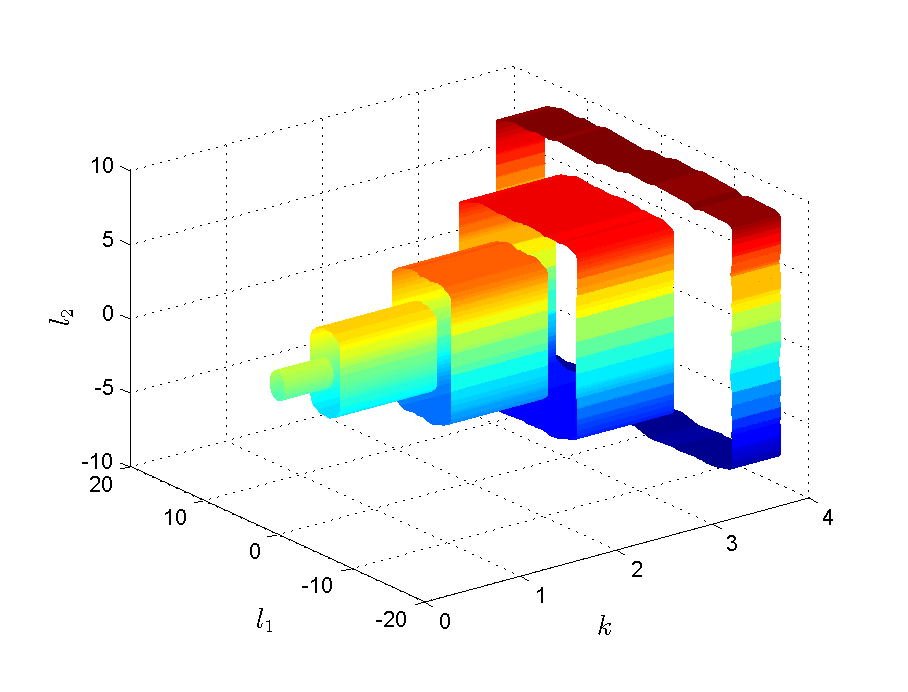
\includegraphics[scale=0.45]{first_stat_3d.eps}
}
\subfigure[Эллипсы в момент $k=4$.]{
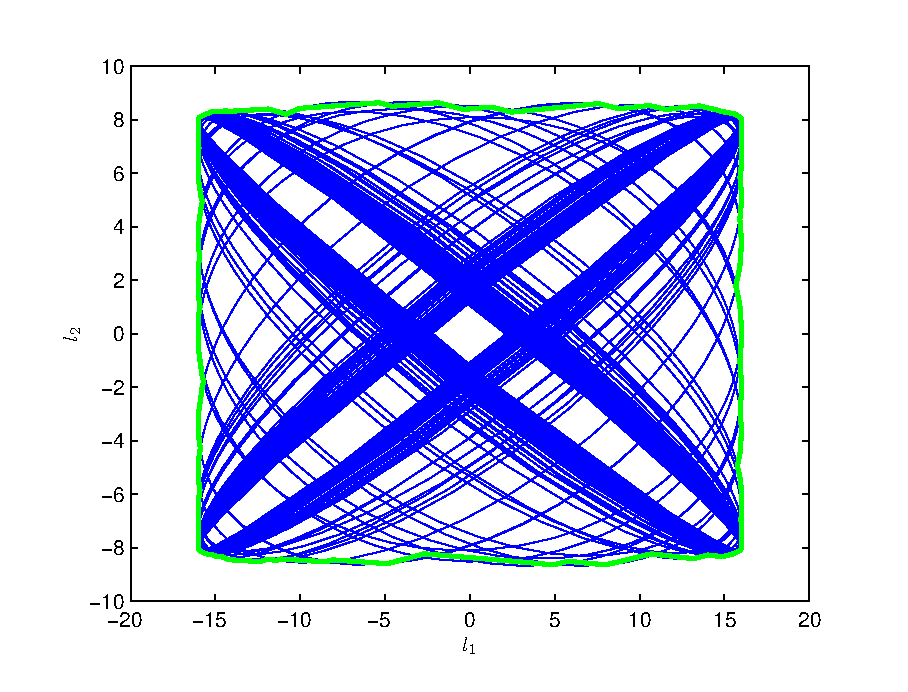
\includegraphics[scale=0.45]{first_stat_2d.eps}
}
\caption{Проекция множества достижимости на статическую плоскость $\left\{(1,0,0,0)',(0,1,0,0)'\right\}$. Количество оценок --- 150.}
\end{figure}

\begin{figure}[H]
\subfigure[Трубка достижимости, $k=0,\dots 4$.]{
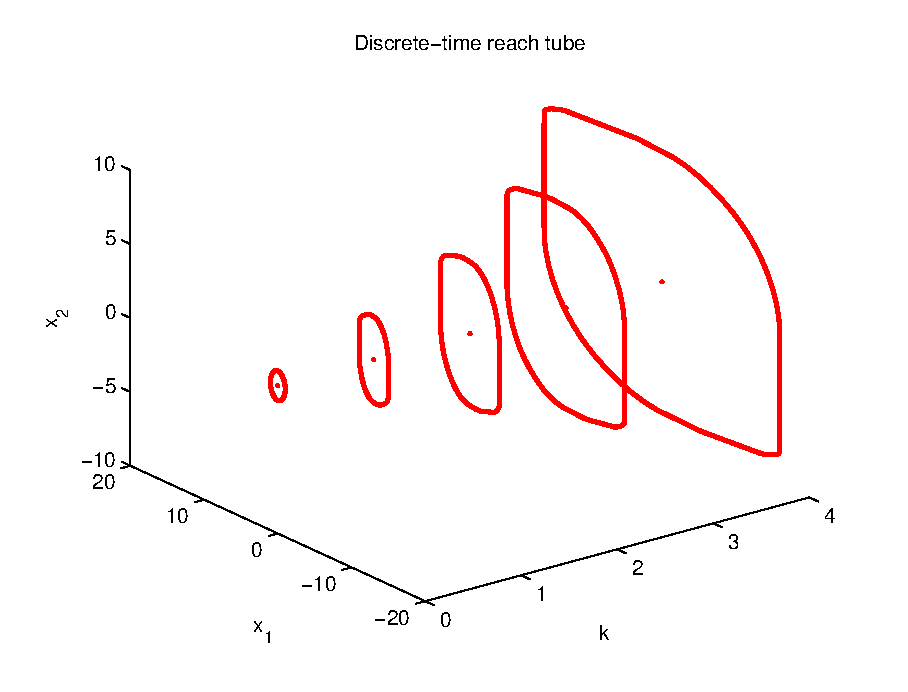
\includegraphics[scale=0.45]{first_tool_3d.eps}
}
\subfigure[Эллипсы в момент $k=4$.]{
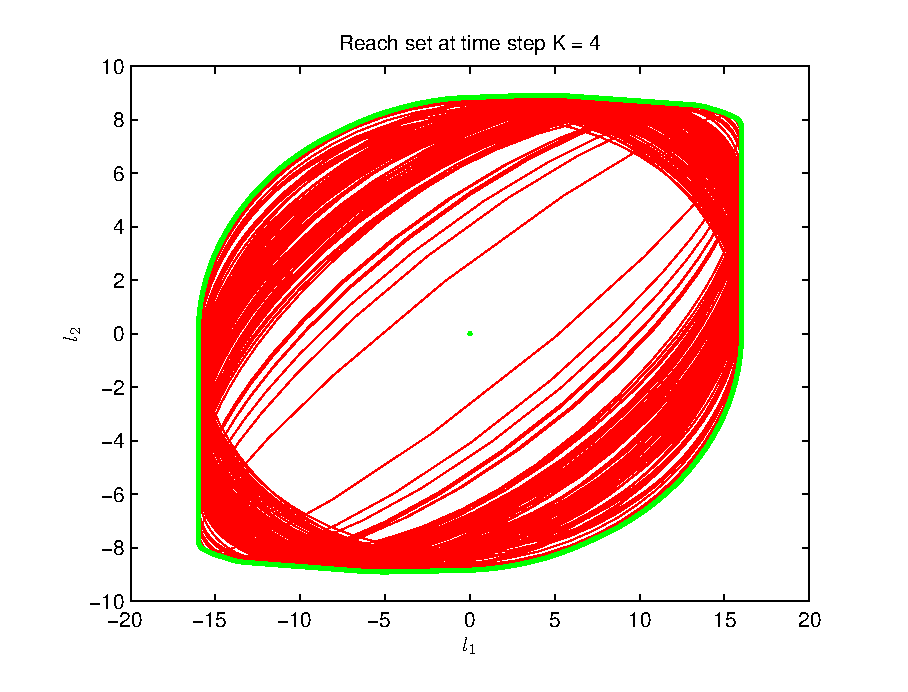
\includegraphics[scale=0.45]{first_tool_2d.eps}
}
\caption{Проекция множества достижимости на статическую плоскость $\left\{(1,0,0,0)',(0,1,0,0)'\right\}$ с помощью ellipsoidal toolbox. Количество оценок --- 100.}
\end{figure}

\begin{figure}[H]
\subfigure[Трубка достижимости, $k=0,\dots 4$.]{
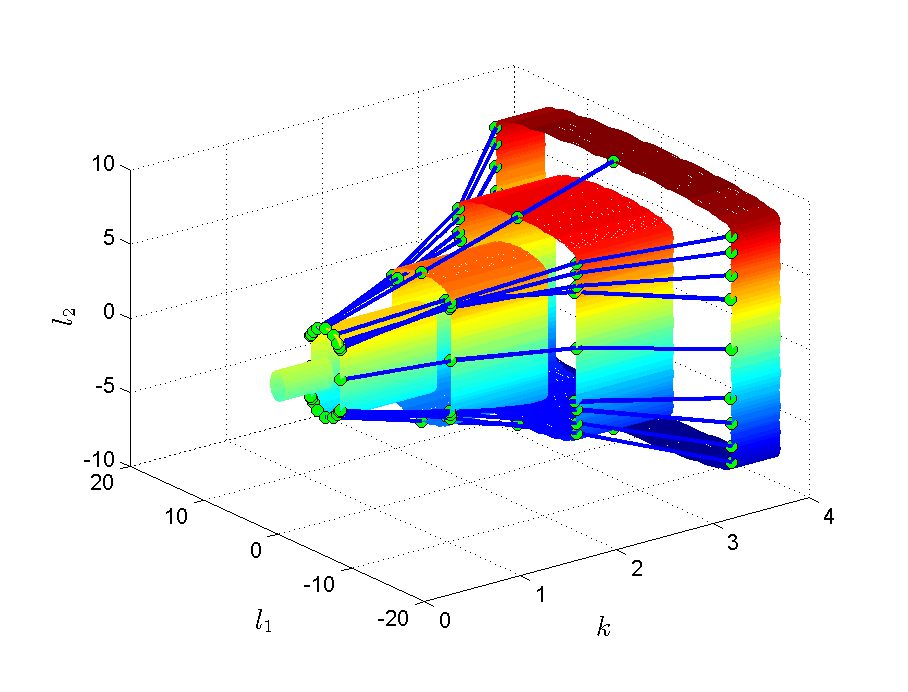
\includegraphics[scale=0.45]{first_dyna_3d.eps}
}
\subfigure[Эллипсы в момент $k=4$.]{
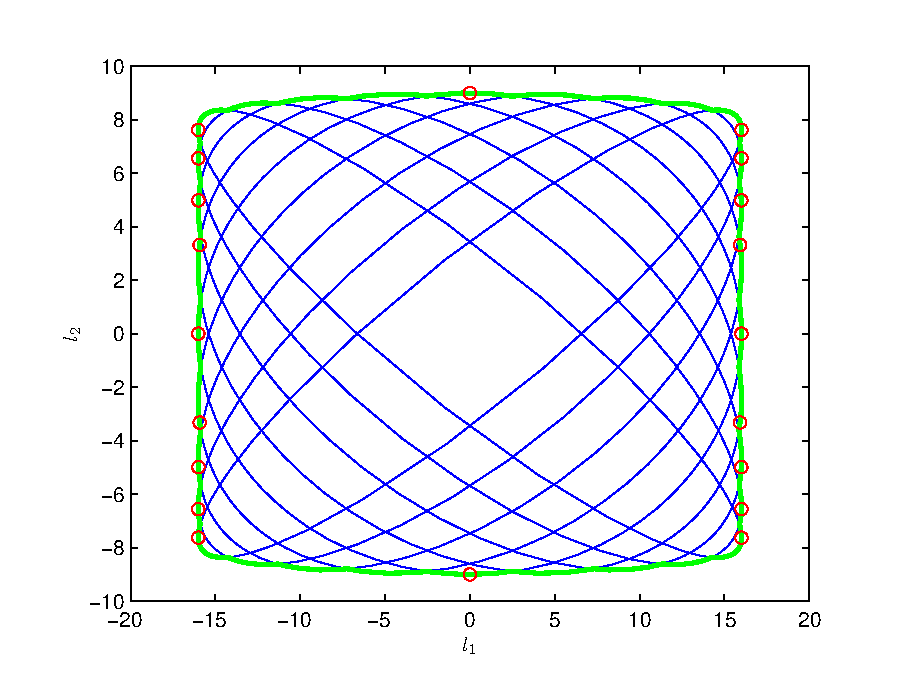
\includegraphics[scale=0.45]{first_dyna_2d.eps}
}
\caption{Проекция множества достижимости на динамическую плоскость с начальными положениями $\left\{(1,0,0,0)',(0,1,0,0)'\right\}$. Количество оценок --- 20.}
\end{figure}

Из вида матриц следует, что система независимо развивается по всем направлениям, причем для первых двух координат верны уравнения:
\begin{gather*}
x_1(k+1) = 2*x_1(k),\\
x_2(k+1) = x_2(k)+2u_2,\quad u_2 \in[-1,1].
\end{gather*}

Отсюда видно, что система границы множества достижимости на каждом следующем шаге увеличиваются по модулю на единицу по $x_2$, и удваиваются по $x_1$. Так как начальный эллипсоид симметричен относительно начала координат и осей $Ox_1, Ox_2$, то и множество достижимости на каждом шаге будет также будет симметрично. Однако рисунок ellipsoidal toolbox если и приближается к симметричному относительно осей виду, то очень медленно. Отсюда следует сделать вывод, что либо в toolbox ошибка, либо слишком мала точность.

\subsection{Пример №2: 3-мерная устойчивая система}
\begin{gather*} A =
\left(\begin{array}{ccc} -0.5 & 1 & 0\\ -1 & 1 & -0.5\\ -1 & 0 & -0.5 \end{array}\right),\quad
B =
\left(\begin{array}{ccc} 1 & 0 & 0\\ 0 & 1 & 0\\ 0 & 0 & 1 \end{array}\right),\quad
X_0 =
\left(\begin{array}{ccc} 1 & 0 & 0\\ 0 & 1 & 0\\ 0 & 0 & 1 \end{array}\right),\quad
x_0 =
\left(\begin{array}{c} 0\\ 0\\ 0 \end{array}\right),\quad \\
Q =
\left(\begin{array}{ccc} 1 & 0 & 0\\ 0 & 1 & 0\\ 0 & 0 & 1 \end{array}\right),\quad
q =
\left(\begin{array}{c} 0\\ 0\\ 0 \end{array}\right).
\end{gather*}

Матрица $A$ в данном примере является устойчивой, так как её собственные значения 
$\{-0.25 + 0.661438i, -0.25 - 0.661438i, 0.5\}$ имеют вещественную часть, по модулю меньшую единицы.

\begin{figure}[H]
\subfigure[Трубка достижимости, $k=0,\dots 4$.]{
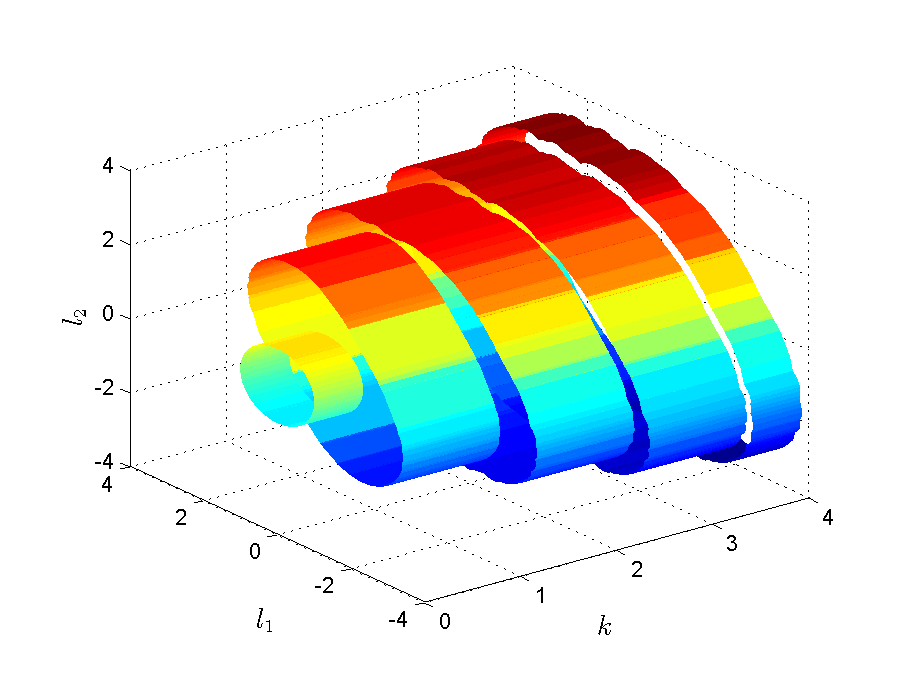
\includegraphics[scale=0.45]{second_stat_3d.eps}
}
\subfigure[Эллипсы в момент $k=4$.]{
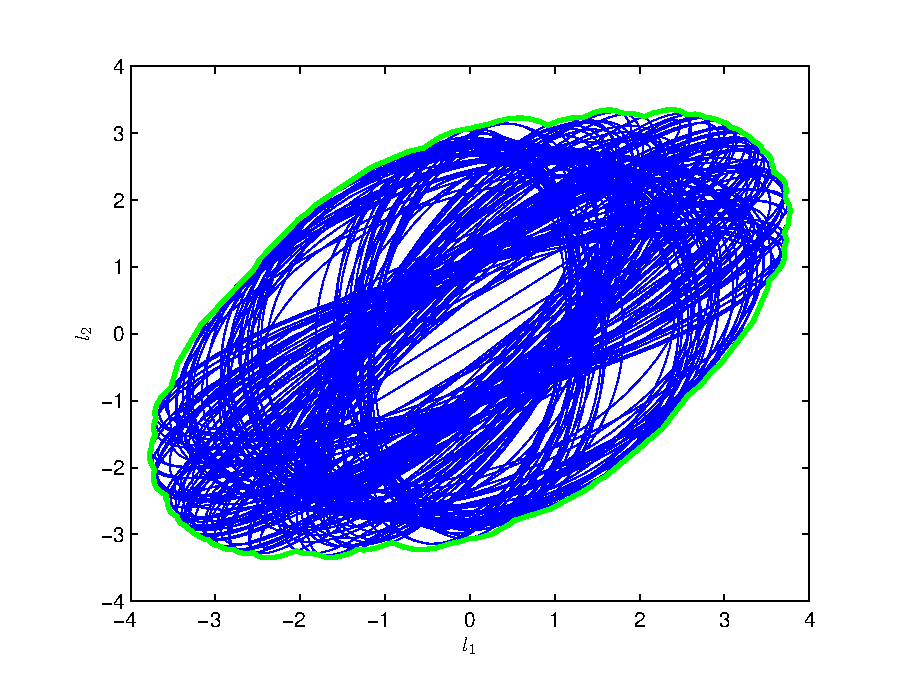
\includegraphics[scale=0.45]{second_stat_2d.eps}
}
\caption{Проекция множества достижимости на статическую плоскость $\left\{(1,0,0)',(0,1,0)'\right\}$. Количество оценок --- 150.}
\end{figure}

\begin{figure}[H]
\subfigure[Трубка достижимости, $k=0,\dots 4$.]{
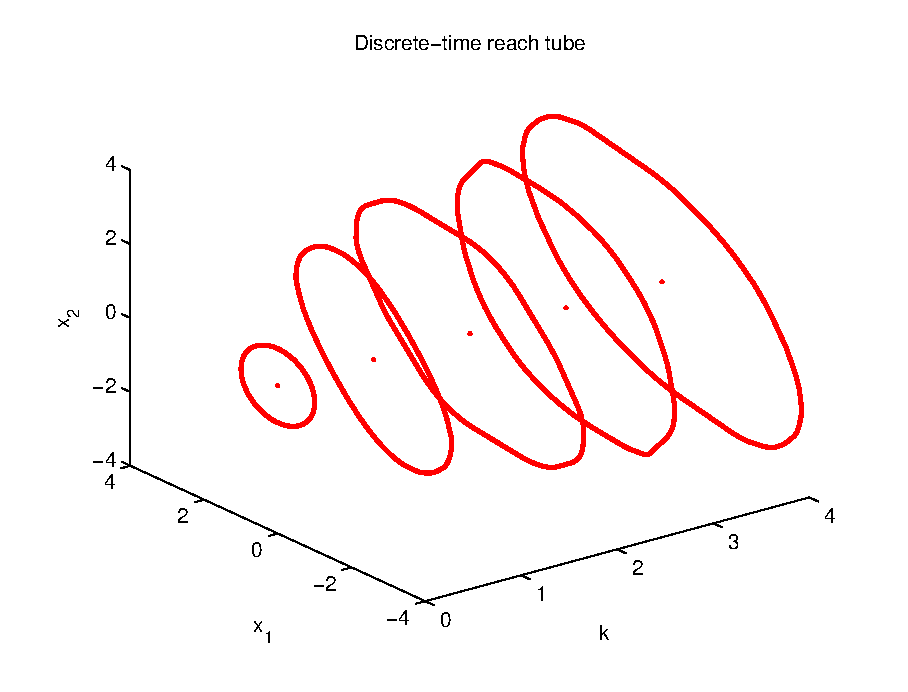
\includegraphics[scale=0.45]{second_tool_3d.eps}
}
\subfigure[Эллипсы в момент $k=4$.]{
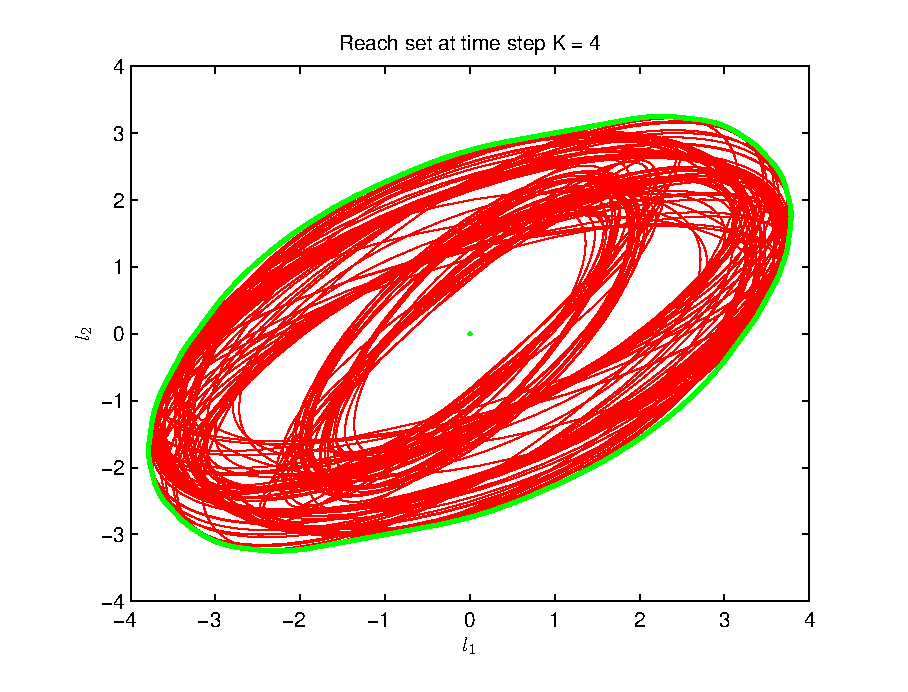
\includegraphics[scale=0.45]{second_tool_2d.eps}
}
\caption{Проекция множества достижимости на статическую плоскость $\left\{(1,0,0)',(0,1,0)'\right\}$ с помощью ellipsoidal toolbox. Количество оценок --- 150.}
\end{figure}

\begin{figure}[H]
\subfigure[Трубка достижимости, $k=0,\dots 4$.]{
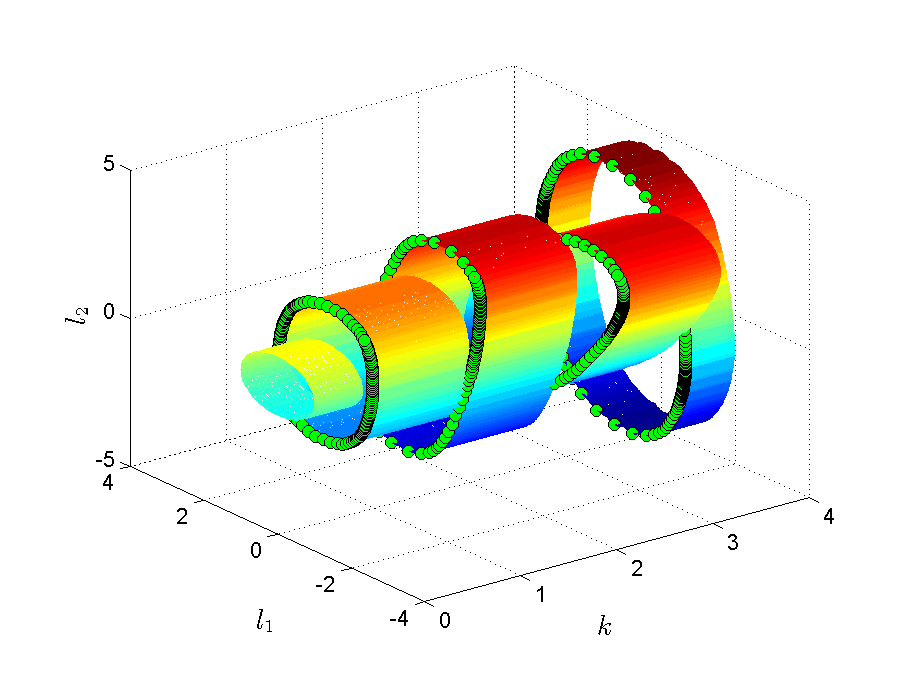
\includegraphics[scale=0.45]{second_dyna_3d.eps}
}
\subfigure[Эллипсы в момент $k=4$.]{
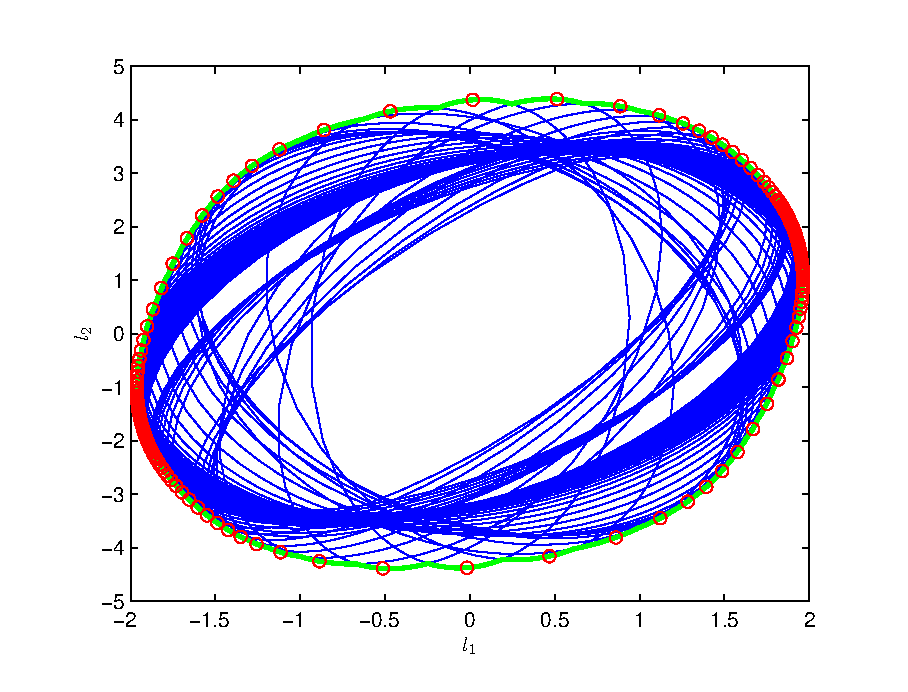
\includegraphics[scale=0.45]{second_dyna_2d.eps}
}
\caption{Проекция множества достижимости на динамическую плоскость с начальными положениями $\left\{(1,0,0)',(0,1,0)'\right\}$. Количество оценок --- 100.}
\end{figure}

Для этого примера характерно следующее: самописной программе, как и ellipsoidal toolbox, чтобы получить достаточно выпуклую фигуру, нужно большое количество направлений оценки, что приводит к большим затратам времени. Решением этой проблемы может быть разработка алгоритма с адаптивной сеткой направлений.

\subsection{Пример №3: 3-мерная неустойчивая система}
\begin{gather*}
A =
\left(\begin{array}{ccc} 2 & 1 & 0\\ -3 & 1 & -0.5\\ -1 & 0 & -2 \end{array}\right),\quad
B =
\left(\begin{array}{ccc} 0.6 & 0.3 & 0.1\\ 0.2 & 0.7 & 0.2\\ 0.5 & 0.1 & 1 \end{array}\right),\quad
X_0 =
\left(\begin{array}{ccc} 2 & 0 & 1\\ 0 & 2 & 0\\ 1 & 0 & 2 \end{array}\right),\quad
x_0 =
\left(\begin{array}{c} 0\\ 0\\ 0 \end{array}\right),\quad \\
Q =
\left(\begin{array}{ccc} 1 & 0 & 0\\ 0 & 1 & 0\\ 0 & 0 & 1 \end{array}\right),\quad
q =
\left(\begin{array}{c} 0\\ 0\\ 0 \end{array}\right).
\end{gather*}

Все собственные значения $\left( \{1.48307 + 1.62245 I, 1.48307 - 1.62245 I, -1.96613\} \right)$ имеют вещественную часть больше единицы, поэтому система неустойчива.

\begin{figure}[H]
\subfigure[Трубка достижимости, $k=0,\dots 8$.]{
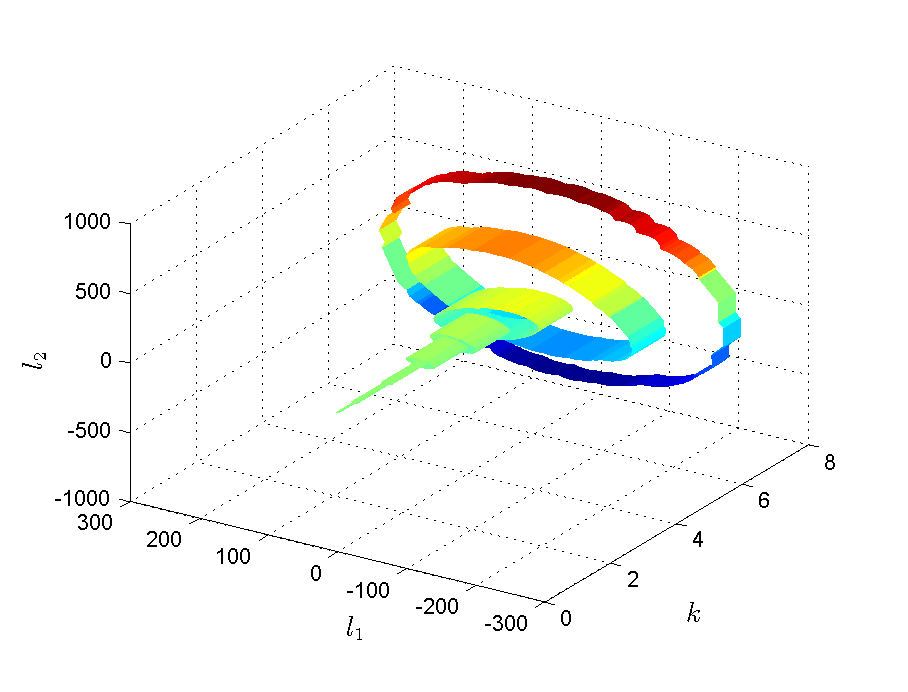
\includegraphics[scale=0.45]{third_stat_3d.eps}
}
\subfigure[Эллипсы в момент $k=8$.]{
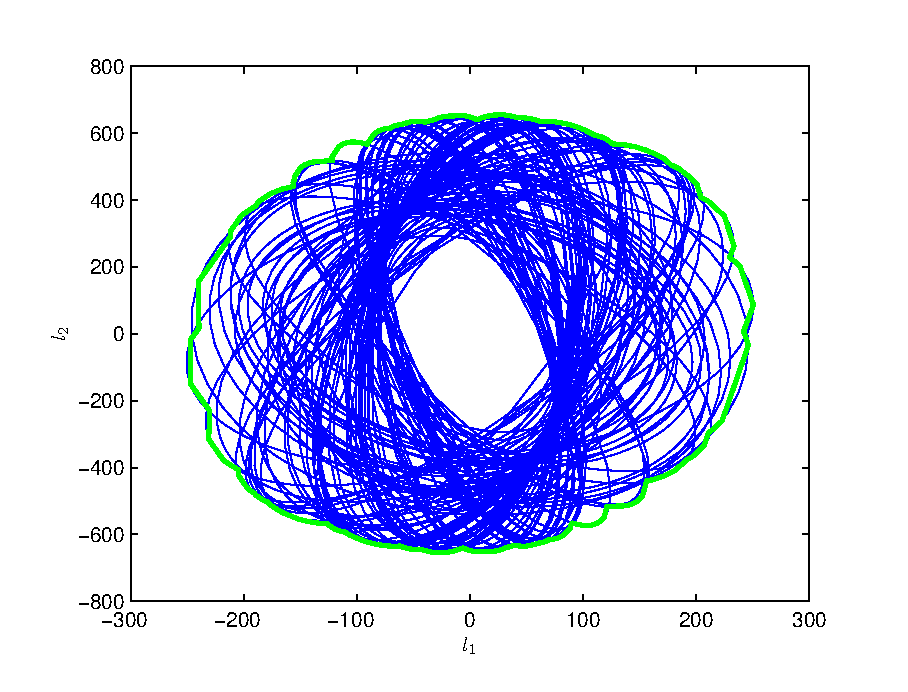
\includegraphics[scale=0.45]{third_stat_2d.eps}
}
\caption{Проекция множества достижимости на статическую плоскость $\left\{(1,0,2)',(1,1,1)'\right\}$. Количество оценок --- 100.}
\end{figure}

\begin{figure}[H]
\subfigure[Трубка достижимости, $k=0,\dots 8$.]{
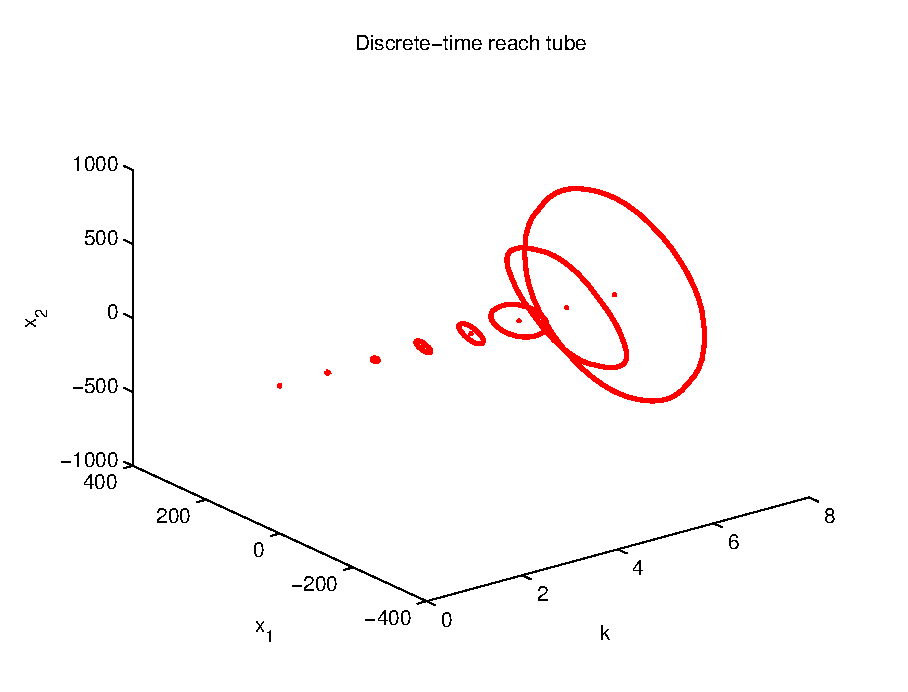
\includegraphics[scale=0.45]{third_tool_3d.eps}
}
\subfigure[Эллипсы в момент $k=8$.]{
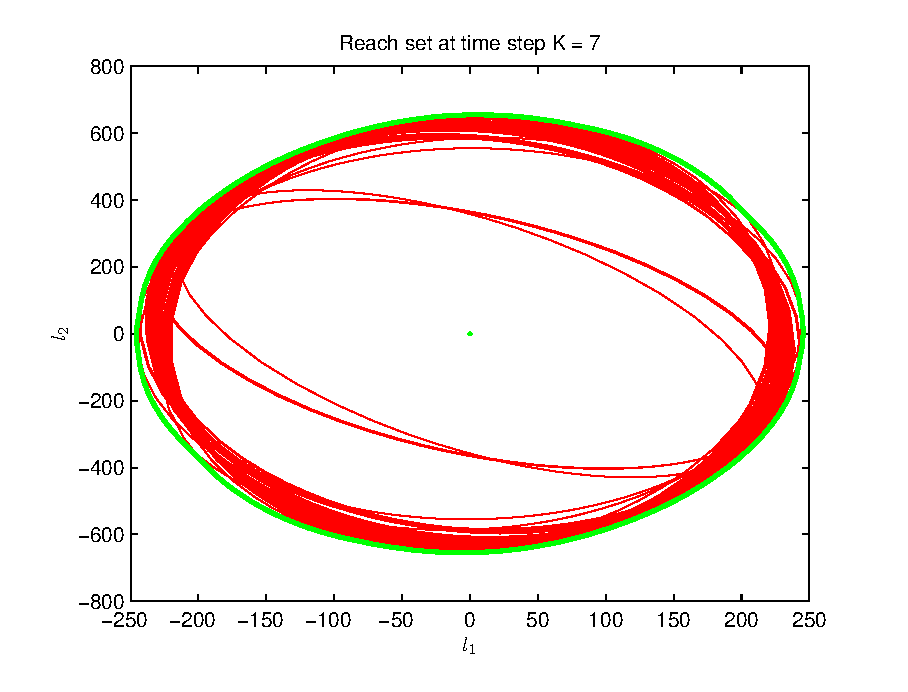
\includegraphics[scale=0.45]{third_tool_2d.eps}
}
\caption{Проекция множества достижимости на статическую плоскость $\left\{(1,0,2)',(1,1,1)'\right\}$ с помощью ellipsoidal toolbox. Количество оценок --- 50.}
\end{figure}

\begin{figure}[H]
\subfigure[Трубка достижимости, $k=0,\dots 8$.]{
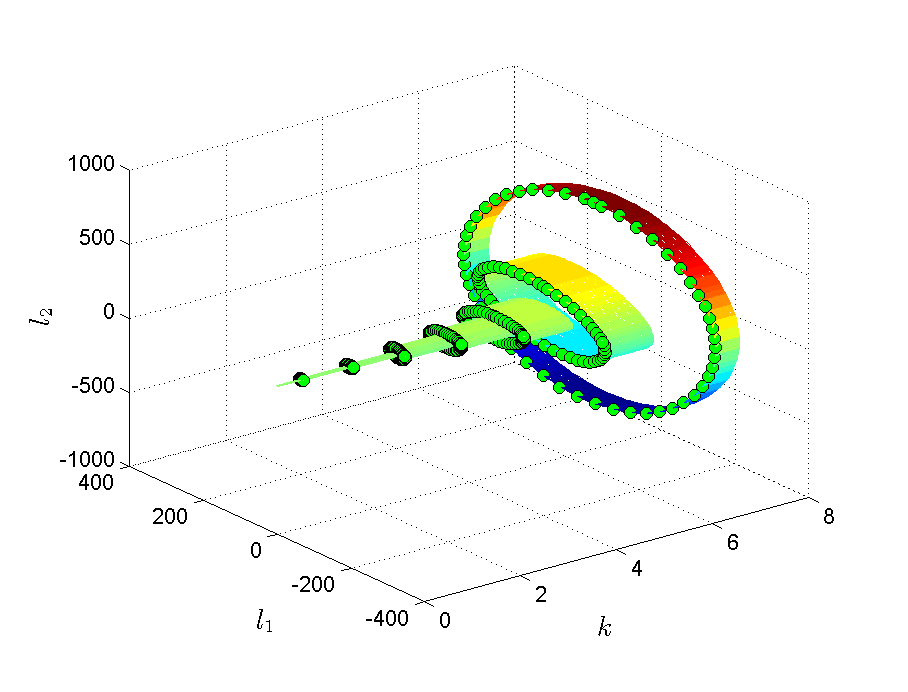
\includegraphics[scale=0.45]{third_dyna_3d.eps}
}
\subfigure[Эллипсы в момент $k=8$.]{
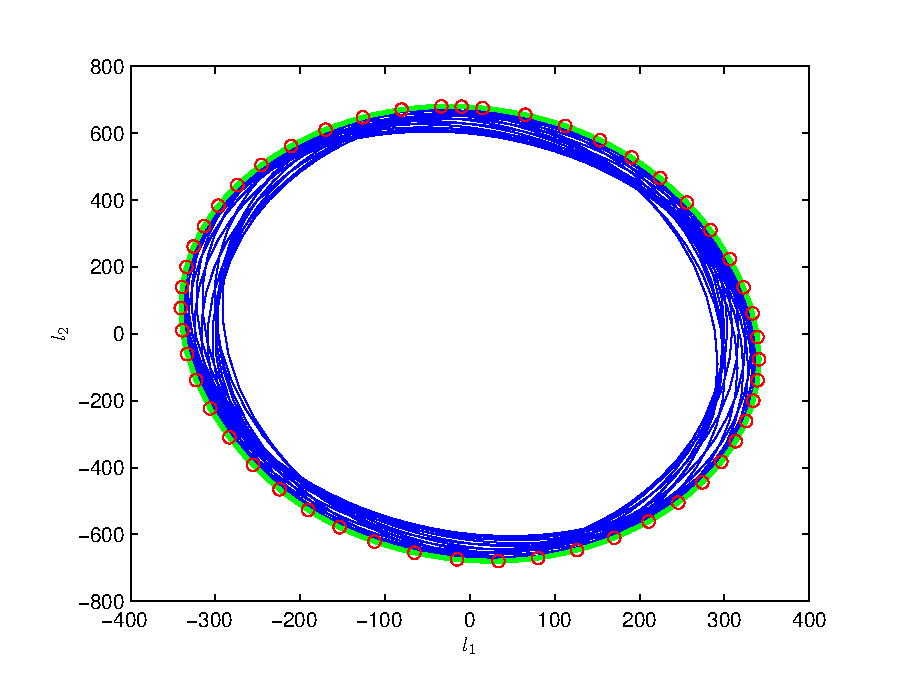
\includegraphics[scale=0.45]{third_dyna_2d.eps}
}
\caption{Проекция множества достижимости на динамическую плоскость с начальными положениями $\left\{(1,0,2)',(1,1,1)'\right\}$. Количество оценок --- 50.}
\end{figure}

\subsection{Пример №4: нулевая матрица B}
\begin{gather*}
A =
\left(\begin{array}{cc} 0.433884 & 0.900969\\ -0.900969 & 0.433884 \end{array}\right),\quad
B =
\left(\begin{array}{cc} 0 & 0\\ 0 & 0 \end{array}\right),\quad
X_0 =
\left(\begin{array}{cc} 16 & 0\\ 0 & 4 \end{array}\right),\quad
x_0 =
\left(\begin{array}{c} 0\\ 0 \end{array}\right),\\
Q =
\left(\begin{array}{cc} 1 & 0\\ 0 & 1 \end{array}\right),\quad
q =
\left(\begin{array}{c} 0\\ 0 \end{array}\right).
\end{gather*}

Программа корректно работает, например, при сингулярной матрице $B$. Результат работы ellipsoidal toolbox не приводится в силу очевидности.

\begin{figure}[H]
\subfigure[Трубка достижимости, $k=0,\dots 8$.]{
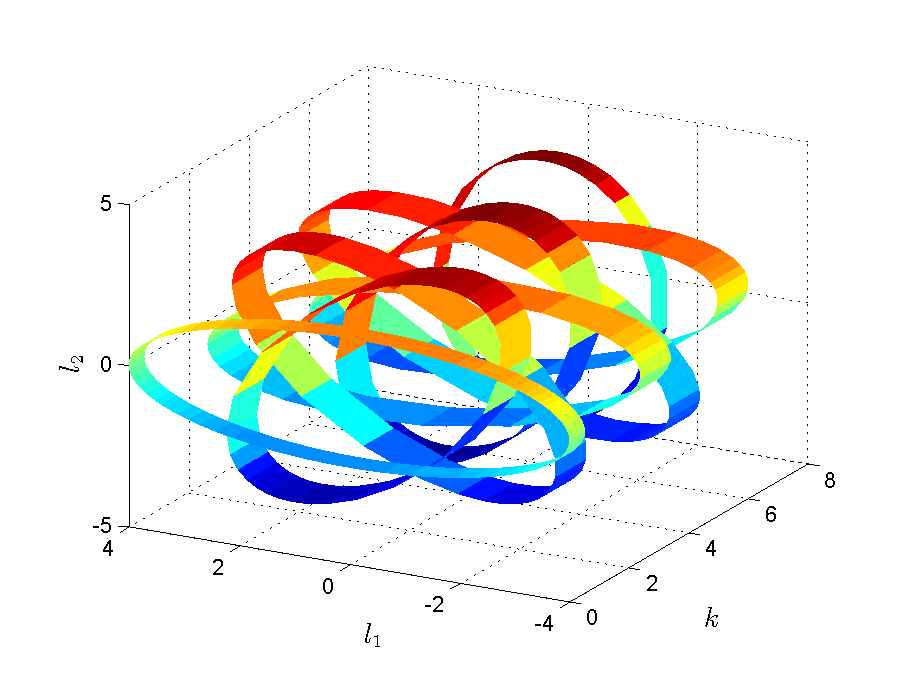
\includegraphics[scale=0.45]{fourth_stat_3d.eps}
}
\subfigure[Эллипсы в момент $k=8$.]{
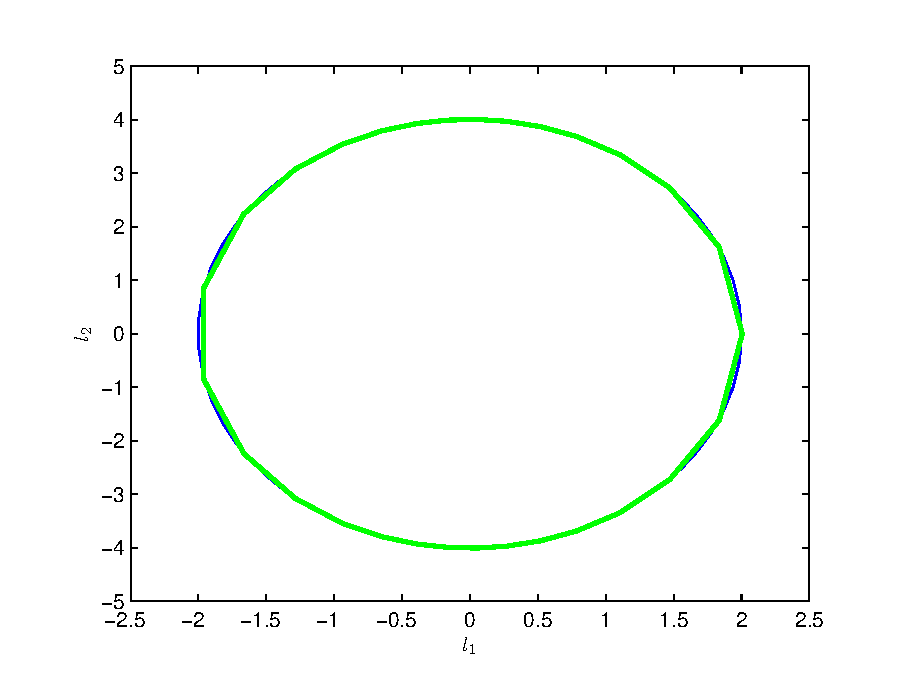
\includegraphics[scale=0.45]{fourth_stat_2d.eps}
}
\caption{Проекция множества достижимости на статическую плоскость $\left\{(1,0)',(0,1)'\right\}$. Количество оценок --- 10.}
\end{figure}

\begin{figure}[H]
\subfigure[Трубка достижимости, $k=0,\dots 8$.]{
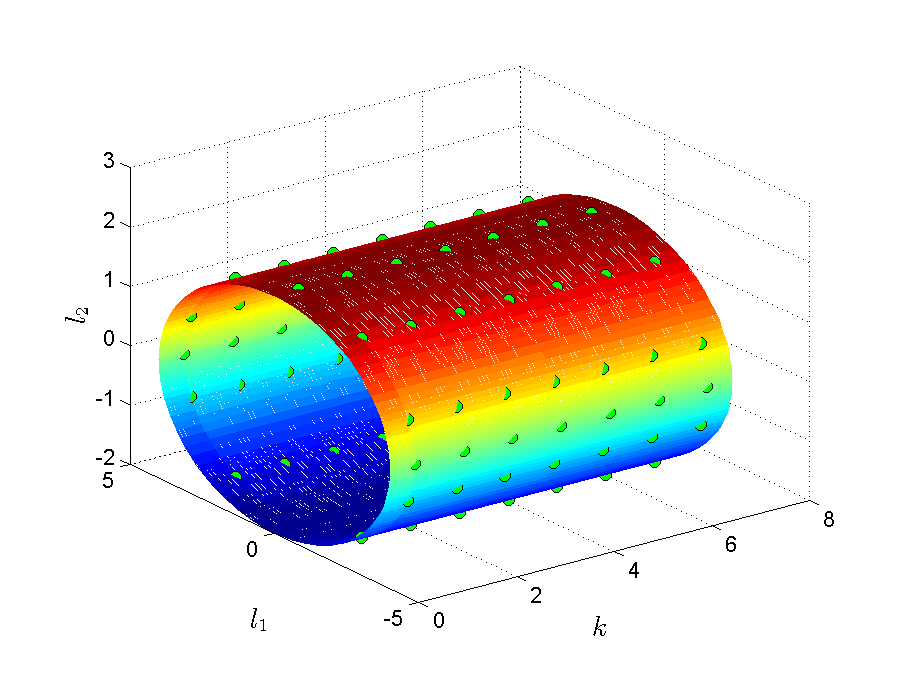
\includegraphics[scale=0.45]{fourth_dyna_3d.eps}
}
\subfigure[Эллипсы в момент $k=8$.]{
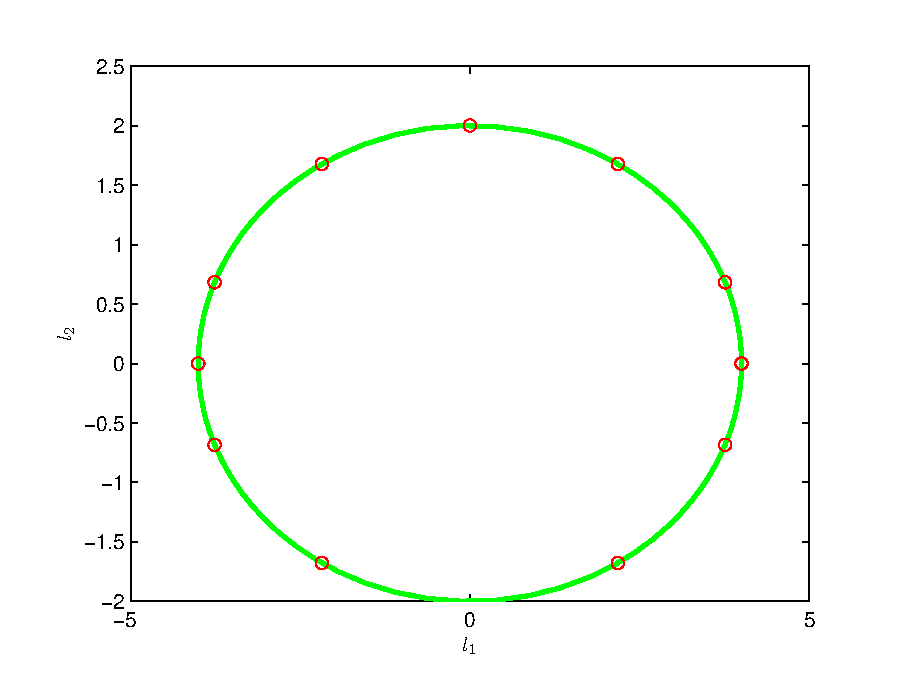
\includegraphics[scale=0.45]{fourth_dyna_2d.eps}
}
\caption{Проекция множества достижимости на динамическую плоскость с начальными положениями $\left\{(1,0,2)',(1,1,1)'\right\}$. Количество оценок --- 10.}
\end{figure}

\subsection{Пример №5: нестационарная система}
\begin{gather*}
A =
\left(\begin{array}{ccc} \sin\!\left(k\right) & 0 & 0\\ 0.75\, \cos\!\left(k\right) & 0 & 0.5\, \cos\!\left(k\right)\\ 0 & \sin\!\left(k\right) & 0 \end{array}\right), \quad
B =
\left(\begin{array}{cc} 0 & 1\\ 1 & 1\\ 2 & 1 \end{array}\right), \quad \\
X_0 =
\left(\begin{array}{ccc} \frac{1}{2} & 0 & 0\\ 0 & 1 & 0\\ 0 & 0 & 2 \end{array}\right), \quad
x_0 =
\left(\begin{array}{c} 0\\ 0\\ 0 \end{array}\right), \quad
Q=
\left(\begin{array}{cc} 2 & 1\\ 1 & 1 \end{array}\right), \quad
q =
\left(\begin{array}{c} 0\\ 0 \end{array}\right).
\end{gather*}

На этом примере вновь видно превосходство точности алгоритма из ellipsoidal toolbox при статической проекции: для достижения выпуклости фигуры в программе в данном случае требуется как минимум 1000 различных направлений. Приведён пример для $350$, поскольку график большего числа эллипсов слишком загромождён.

\begin{figure}[H]
\subfigure[Трубка достижимости, $k=1,\dots 5$.]{
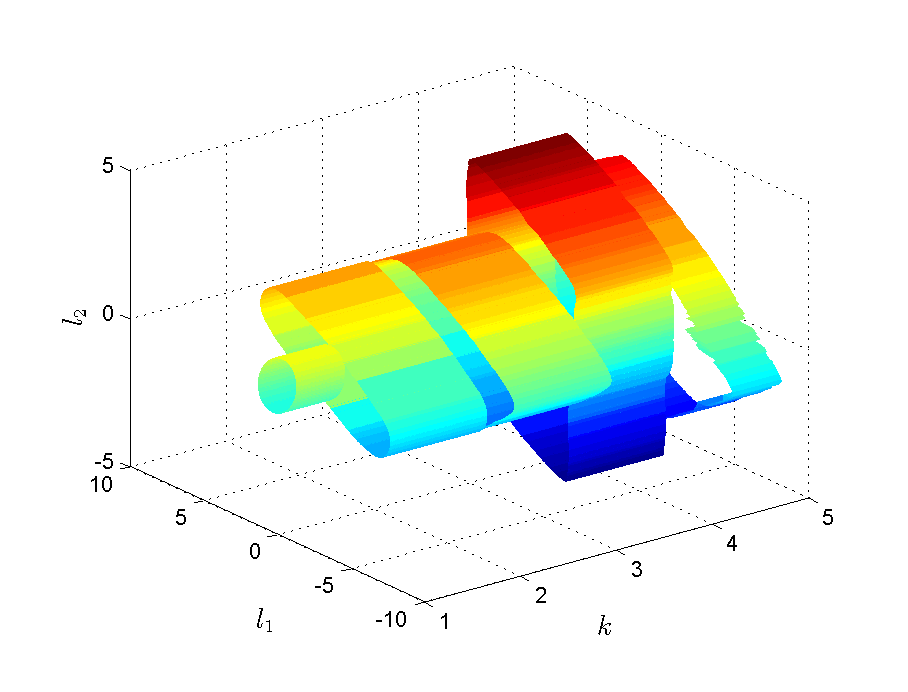
\includegraphics[scale=0.45]{fifth_stat_3d.eps}
}
\subfigure[Эллипсы в момент $k=5$.]{
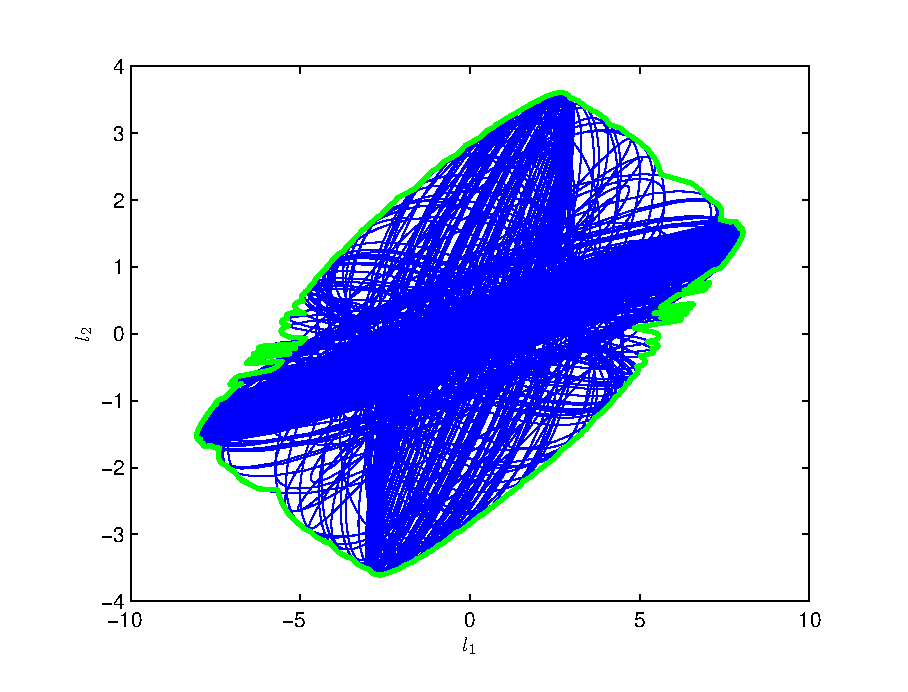
\includegraphics[scale=0.45]{fifth_stat_2d.eps}
}
\caption{Проекция множества достижимости на статическую плоскость $\left\{(1,0,2)',(2,2,1)'\right\}$. Количество оценок --- 350.}
\end{figure}

\begin{figure}[H]
\subfigure[Трубка достижимости, $k=1,\dots 5$.]{
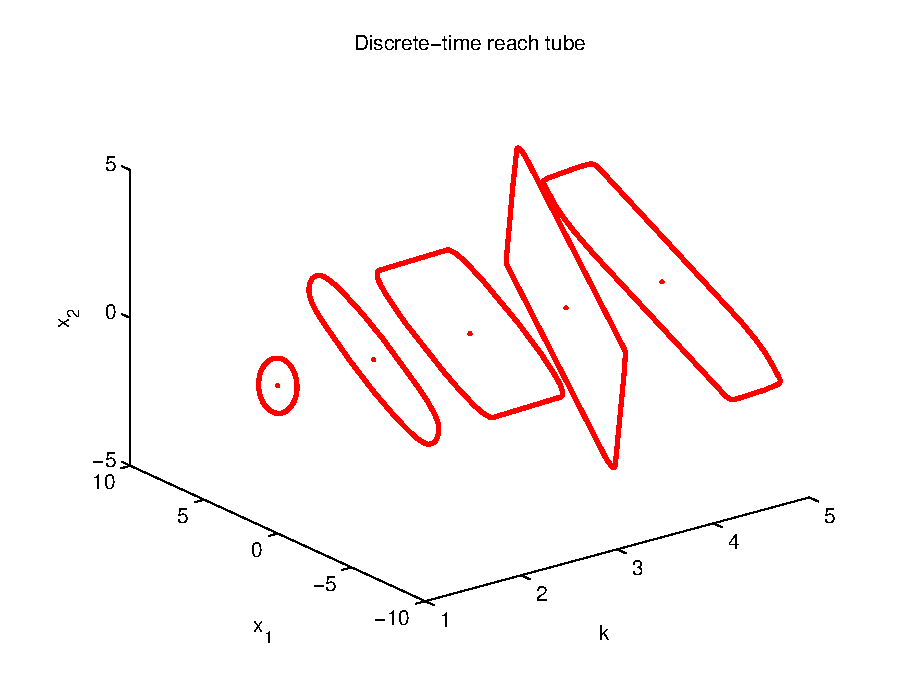
\includegraphics[scale=0.45]{fifth_tool_3d.eps}
}
\subfigure[Эллипсы в момент $k=5$.]{
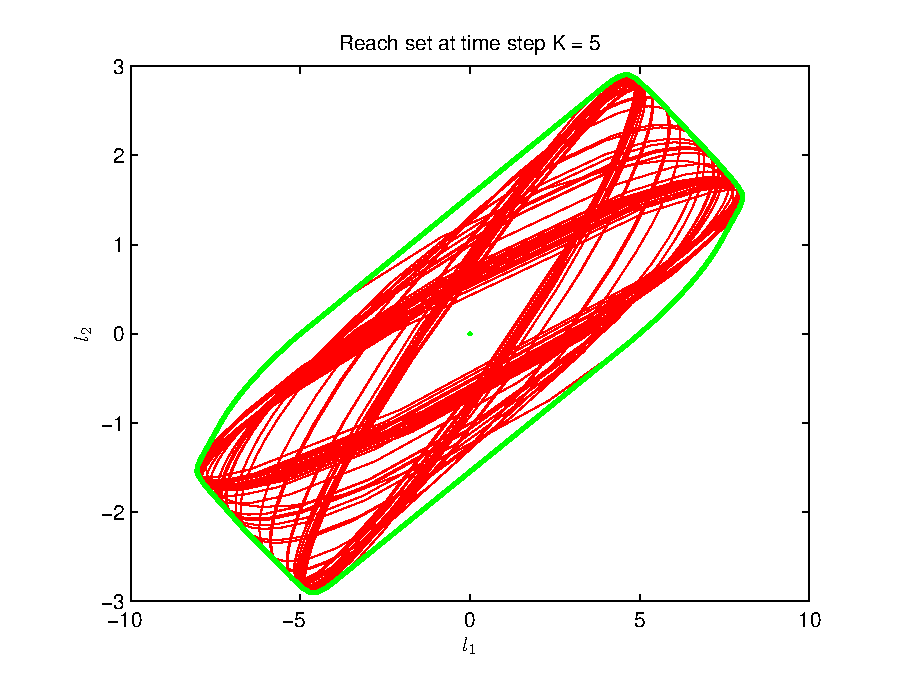
\includegraphics[scale=0.45]{fifth_tool_2d.eps}
}
\caption{Проекция множества достижимости на статическую плоскость $\left\{(1,0,2)',(2,2,1)'\right\}$ с помощью ellipsoidal toolbox. Количество оценок --- 50.}
\end{figure}

\begin{figure}[H]
\subfigure[Трубка достижимости, $k=1,\dots 5$.]{
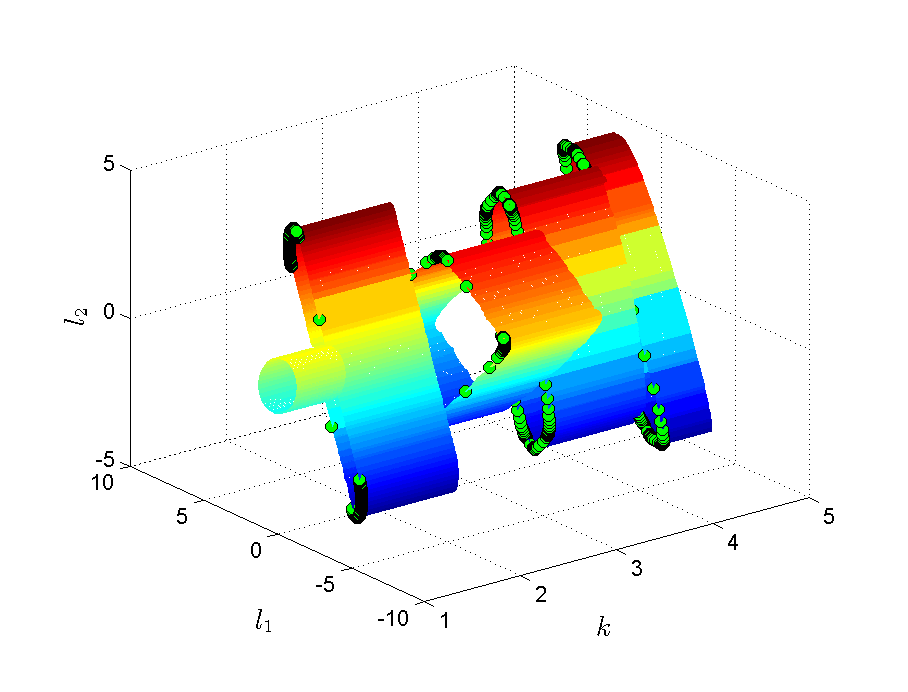
\includegraphics[scale=0.45]{fifth_dyna_3d.eps}
}
\subfigure[Эллипсы в момент $k=5$.]{
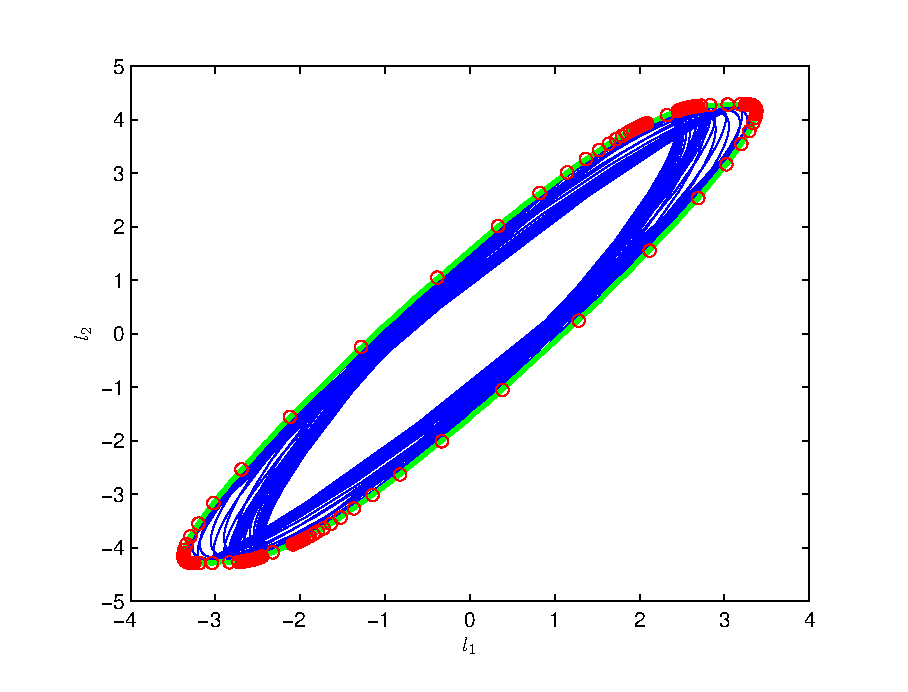
\includegraphics[scale=0.45]{fifth_dyna_2d.eps}
}
\caption{Проекция множества достижимости на динамическую плоскость с начальными положениями $\left\{(1,0,2)',(2,2,1)'\right\}$. Количество оценок --- 150.}
\end{figure}
\section{Сравнение скоростей}
Взяв за единицу скорость поиска одной эллипсоидальной оценки для системы размерности 3 (примерно $0.14$ секунды), были получены следующие относительные результаты:
\begin{tabular}{|l|l|l|l|l|l|l|l|l|l|l|}
\hline
Размерность & 3 & 5 & 10 & 25 & 50 & 100 & 150 & 200 & 250 & 300 \\
\hline
Время работы ET & 1 & 1.1 & 1.3 & 1.5 & 3.1 &  5.8 & 9.4 & 14 & 29.5 & 64 \\
\hline
Время работы не ET & 2.7 & 3 & 4 & 5.2 & 12.5 & 40 & 73 & 124 & 250 & 760 \\
\hline
\end{tabular}

Видно, что ellipsoidal toolbox, не считая проблем из примера 1, значительно лучше оптимизирован, чем написанная для практикума программа.

\newpage

\addcontentsline{toc}{section}{Список литературы}
\bibliographystyle{sastyle}
\nocite{Kurzhanskiy:EECS-2006-46}
\nocite{Kurzhan_varaiya_discrete}
\bibliography{library}


\end{document}